\documentclass[onesided]{article}\usepackage[]{graphicx}\usepackage[]{color}
% maxwidth is the original width if it is less than linewidth
% otherwise use linewidth (to make sure the graphics do not exceed the margin)
\makeatletter
\def\maxwidth{ %
  \ifdim\Gin@nat@width>\linewidth
    \linewidth
  \else
    \Gin@nat@width
  \fi
}
\makeatother

\definecolor{fgcolor}{rgb}{0.345, 0.345, 0.345}
\newcommand{\hlnum}[1]{\textcolor[rgb]{0.686,0.059,0.569}{#1}}%
\newcommand{\hlstr}[1]{\textcolor[rgb]{0.192,0.494,0.8}{#1}}%
\newcommand{\hlcom}[1]{\textcolor[rgb]{0.678,0.584,0.686}{\textit{#1}}}%
\newcommand{\hlopt}[1]{\textcolor[rgb]{0,0,0}{#1}}%
\newcommand{\hlstd}[1]{\textcolor[rgb]{0.345,0.345,0.345}{#1}}%
\newcommand{\hlkwa}[1]{\textcolor[rgb]{0.161,0.373,0.58}{\textbf{#1}}}%
\newcommand{\hlkwb}[1]{\textcolor[rgb]{0.69,0.353,0.396}{#1}}%
\newcommand{\hlkwc}[1]{\textcolor[rgb]{0.333,0.667,0.333}{#1}}%
\newcommand{\hlkwd}[1]{\textcolor[rgb]{0.737,0.353,0.396}{\textbf{#1}}}%
\let\hlipl\hlkwb

\usepackage{framed}
\makeatletter
\newenvironment{kframe}{%
 \def\at@end@of@kframe{}%
 \ifinner\ifhmode%
  \def\at@end@of@kframe{\end{minipage}}%
  \begin{minipage}{\columnwidth}%
 \fi\fi%
 \def\FrameCommand##1{\hskip\@totalleftmargin \hskip-\fboxsep
 \colorbox{shadecolor}{##1}\hskip-\fboxsep
     % There is no \\@totalrightmargin, so:
     \hskip-\linewidth \hskip-\@totalleftmargin \hskip\columnwidth}%
 \MakeFramed {\advance\hsize-\width
   \@totalleftmargin\z@ \linewidth\hsize
   \@setminipage}}%
 {\par\unskip\endMakeFramed%
 \at@end@of@kframe}
\makeatother

\definecolor{shadecolor}{rgb}{.97, .97, .97}
\definecolor{messagecolor}{rgb}{0, 0, 0}
\definecolor{warningcolor}{rgb}{1, 0, 1}
\definecolor{errorcolor}{rgb}{1, 0, 0}
\newenvironment{knitrout}{}{} % an empty environment to be redefined in TeX

\usepackage{alltt}
\usepackage[T1]{fontenc}
\linespread{1.5} % Line spacing - Palatino needs more space between lines
\usepackage{microtype} % Slightly tweak font spacing for aesthetics

\usepackage[hmarginratio=1:1,columnsep=20pt]{geometry} % Document margins
%\usepackage{multicol} % Used for the two-column layout of the document
\usepackage[hang, small,labelfont=bf,up,textfont=it,up]{caption} % Custom captions under/above floats in tables or figures
\usepackage{booktabs} % Horizontal rules in tables
\usepackage{float} % Required for tables and figures in the multi-column environment - they need to be placed in specific locations with the [H] (e.g. \begin{table}[H])

\usepackage{lettrine} % The lettrine is the first enlarged letter at the beginning of the text
\usepackage{paralist} % Used for the compactitem environment which makes bullet points with less space between them

% to ignore texts: good for thank messages and paper submissions.
      % \fbox{\phantom{This text will be invisible too, but a box will be printed arround it.}}

\usepackage{abstract} % Allows abstract customization
\renewcommand{\abstractnamefont}{\normalfont\bfseries} % Set the "Abstract" text to bold
%\renewcommand{\abstracttextfont}{\normalfont\small\itshape} % Set the abstract itself to small italic text

\usepackage[]{titlesec} % Allows customization of titles
\renewcommand\thesection{\Roman{section}} % Roman numerals for the sections
\renewcommand\thesubsection{\Roman{subsection}} % Roman numerals for subsections
\titleformat{\section}[block]{\large\scshape\centering}{\thesection.}{1em}{} % Change the look of the section titles
\titleformat{\subsection}[block]{\large}{\thesubsection.}{1em}{} % Change the look of the section titles

\usepackage{fancybox, fancyvrb, calc}
\usepackage[svgnames]{xcolor}
\usepackage{epigraph}

\usepackage{longtable}
\usepackage{pdflscape}
\usepackage{graphics}

\usepackage{amsfonts}
\usepackage{amsmath}
\usepackage{amssymb}
\usepackage{rotating}
\usepackage{paracol}
\usepackage{textcomp}
\usepackage[export]{adjustbox}
\usepackage{afterpage}
\usepackage{filecontents}
\usepackage{color}
\usepackage{latexsym}
\usepackage{lscape}       %\begin{landscape} and \end{landscape}
\usepackage{wasysym}
\usepackage{dashrule}

\usepackage{framed}
\usepackage{tree-dvips}
\usepackage{pgffor}
\usepackage[]{authblk}
\usepackage{setspace}
\usepackage{array}
\usepackage[latin1]{inputenc}
\usepackage{hyperref}     %desactivar para link rojos
\usepackage{graphicx}
\usepackage{dcolumn} % for R tables
\usepackage{multirow} % For multirow in tables
\usepackage{pifont}
\usepackage{listings}




% hypothesis / theorem package begin
\usepackage{amsthm}
\usepackage{thmtools}
\declaretheoremstyle[
spaceabove=6pt, spacebelow=6pt,
headfont=\normalfont\bfseries,
notefont=\mdseries, notebraces={(}{)},
bodyfont=\normalfont,
postheadspace=0.6em,
headpunct=:
]{mystyle}
\declaretheorem[style=mystyle, name=Hypothesis, preheadhook={\renewcommand{\thehyp}{H\textsubscript{\arabic{hyp}}}}]{hyp}

\usepackage{cleveref}
\crefname{hyp}{hypothesis}{hypotheses}
\Crefname{hyp}{Hypothesis}{Hypotheses}
% hypothesis / theorem package end


%----------------------------------------------------------------------------------------
% Other ADDS-ON
%----------------------------------------------------------------------------------------

% independence symbol \independent
\newcommand\independent{\protect\mathpalette{\protect\independenT}{\perp}}
\def\independenT#1#2{\mathrel{\rlap{$#1#2$}\mkern2mu{#1#2}}}







\hypersetup{
    bookmarks=true,         % show bookmarks bar?
    unicode=false,          % non-Latin characters in Acrobat's bookmarks
    pdftoolbar=true,        % show Acrobat's toolbar?
    pdfmenubar=true,        % show Acrobat's menu?
    pdffitwindow=true,     % window fit to page when opened
    pdfstartview={FitH},    % fits the width of the page to the window
    pdftitle={My title},    % title
    pdfauthor={Author},     % author
    pdfsubject={Subject},   % subject of the document
    pdfcreator={Creator},   % creator of the document
    pdfproducer={Producer}, % producer of the document
    pdfkeywords={keyword1} {key2} {key3}, % list of keywords
    pdfnewwindow=true,      % links in new window
    colorlinks=true,       % false: boxed links; true: colored links
    linkcolor=Maroon,          % color of internal links (change box color with linkbordercolor)
    citecolor=Maroon,        % color of links to bibliography
    filecolor=Maroon,      % color of file links
    urlcolor=Maroon           % color of external links
}

%\usepackage[nodayofweek,level]{datetime} % to have date within text

\newcommand{\LETT}[3][]{\lettrine[lines=4,loversize=.2,#1]{\smash{#2}}{#3}} % letrine customization



% comments on margin
  % Select what to do with todonotes: 
  % \usepackage[disable]{todonotes} % notes not showed
  \usepackage[draft]{todonotes}   % notes showed
  % usage: \todo{This is a note at margin}

\usepackage{cooltooltips}

%%% bib begin
\usepackage[american]{babel}
\usepackage{csquotes}
\usepackage[backend=biber,style=authoryear,dashed=false,doi=false,isbn=false,url=false,arxiv=false]{biblatex}
%\DeclareLanguageMapping{american}{american-apa}
\addbibresource{Vote_Selling_Bahamonde_Canales.bib} 
% USAGES
%% use \textcite to cite normal
%% \parencite to cite in parentheses
%% \footcite to cite in footnote
%% the default can be modified in autocite=FOO, footnote, for ex. 
%%% bib end


% DOCUMENT ID



% TITLE SECTION

\title{\vspace{-15mm}\fontsize{18pt}{7pt}\selectfont\textbf{\input{title.txt}\unskip}} % Article title


\author[1]{

\textsc{H\'ector Bahamonde}
\thanks{\href{mailto:hector.bahamonde@uoh.cl}{hector.bahamonde@uoh.cl}; \href{http://www.hectorbahamonde.com}{\texttt{www.HectorBahamonde.com}}.}}



\author[2]{

\textsc{Andrea Canales}
\thanks{\href{mailto:andrea.canales@uoh.cl}{andrea.canales@uoh.cl}; 
\href{https://www.uoh.cl}{\texttt{website}}. \\
We thank O'Higgins University for funding this project, and the participants of the colloquium at the Centre for Experimental Social Sciences (CESS) at Universidad de Santiago. Javiera Tobar, Cristopher Reyes and Bastian Garrido provided excellent research assistance.}}


\affil[1]{Assistant Professor, O$'$Higgins University (Chile)}
\affil[2]{Postdoctoral Fellow, O$'$Higgins University (Chile)}


\date{\today}

%----------------------------------------------------------------------------------------
\IfFileExists{upquote.sty}{\usepackage{upquote}}{}
\begin{document}
\pagenumbering{gobble} 


\setcounter{hyp}{0} % sets hypothesis counter to 1

\maketitle % Insert title


%----------------------------------------------------------------------------------------
% ABSTRACT
%----------------------------------------------------------------------------------------

%%%%%%%%%%%%%%%%%%%%%%%%%%%%%%%%%%%%%%%%%%%%%%
% begin knitr stuff



% end knitr stuff
%%%%%%%%%%%%%%%%%%%%%%%%%%%%%%%%%%%%%%%%%%%%%%


\begin{abstract}
\input{abstract.txt}\unskip
\end{abstract}

\hspace*{1.3cm}{\bf Please consider downloading the last version of the paper} \href{https://github.com/hbahamonde/Economic_Experiment_Vote_Selling/raw/master/Vote_Selling_Bahamonde_Canales_Paper.pdf}{\texttt{{\color{red}here}}}.

\providecommand{\keywords}[1]{\textbf{\textit{Keywords---}} #1} % keywords.  
\keywords{clientelism; vote-buying; vote-selling; experimental economics; formal modeling.}



%%%%%%%%%%%%%%%%%%%%%%%%%%%%%%%%%%%%%%%%%%%%%%
% CONTENT (write the paper below)
%%%%%%%%%%%%%%%%%%%%%%%%%%%%%%%%%%%%%%%%%%%%%%
\clearpage
\newpage
\pagenumbering{arabic}
\setcounter{page}{1}


\section{Introduction}

Nice introduction here. This is my edition.

\section{The Model}
We consider an electorate of $n$ voters. Voters vote for a leader to implement a common policy $\gamma$ from the set $\Gamma=\{1,2,...,100\}$. Each citizen $i$ has an ideal point $x_i$ which is an \emph{iid} draw from an uniform distribution $\Gamma$. When policy $\gamma$ is implemented, payoffs of citizen $i$ are given by $u(D,x_i,\gamma)=D-\vert x_i-\gamma \vert$, where $D$ represents \textcolor{red}{completar ac\'a}. This payoff can be incremented by transferences from both parties to voter $i$.

In this election, there are two candidates. One ``left-wing'' party and one ``right-wing'' party. The left-wing (right-wing) candidate represents a policy $\gamma_L$ ($\gamma_R$) which is an \emph{iid} draw from an uniform distribution over $\{1,...,50\}$ ($\{51,...,100\}$). The location of this policy give us the number of voters $n_L$ leaning towards the left-wing candidate, while the number of voters leaning towards the right-wing party is given by $n_L+n_R=n$. While we consider that voters are attached to an ideological continuum, we do so with the sole purpose of modeling preferences. 

Ultimately, experimental subjects are not told anything about ideology. They only observe that there are a number of ``points'' associated with the victory of party A or party B. In this sense, voters lean (``ideologically'') towards the party that gives them more points.\todo{Andre: check re-wording. Does it still make sense?}
\todo[color=red]{esto de los puntos lo eliminar�a, porque es m�s del dise�o experimental}

Moving forward, both parties negotiate with only one of these $n$ voters. That voter is randomly selected from the total population $n$. Observe that the higher the $n$, the lower the representation in the election of this voter. That is, a larger $n$ necessarily implies that every individual electoral choice matters less. {\color{red}However, if $n$ is small, negotiating with this voter may be more attractive to political parties}.\todo{por que? no lo hace mas caro? (dictador)}
\todo[color=red]{Porque en este caso, cada votante representa un mayor porcentaje de la poblaci�n total.}
We assume that each candidate has a budget ($B$) that they can use to buy votes. If a party decides not to negotiate with the voter (or the voter does no accept the offer), the party keeps this budget. The profits of party $i$ is given by,

\begin{align*}
  \pi_i(W,e_i,s_i)=W\cdot e_i+(1-s_i\cdot a_j )\cdot B
\end{align*}

where $W$ ($W\geq B$) is a constant that represents how much each party values winning the election, $e_i=1$ if party $i$ wins the election, 0 otherwise,  $s_i$ is the fraction of $B$ that the party offers to voter $j$ who can accept the offer ($a_j=1$) or not ($a_j=0$). We study two versions of this party-voter interaction. One is where both parties make simultaneous offers to the voter, and she decides whether to accept the offer (vote-buying case). Another one is where the voter can make private\todo{por que private? } \todo[color=red]{Porque cuando negocian con cada partido, el otro partido no sabe si el votante est� negociando con el otro partido, ni qu� est� negociando.} offers to both parties, and then the party decides if to pay or not for that voter's vote (vote-selling case).

The timing of the game is as follows: at the beginning of the game $n$ voters and two political parties are randomly located on their respective ideal points: voters along $\Gamma$, the ``left-wing'' candidate along $\{1,...,50\}$, and the ``right-wing'' candidate on $\{51,...,100\}$. All locations are public information, as well as {\color{red}every party's budget} $B$\todo{es asi?} \todo[color=red]{si}, the total number of voters ($n$) and the number of supporters of each party ($n_L$ and $n_R$). What follows then, depends on the specific game. On the vote-buying case, each party simultaneously decides if making an offer to the voter. If a party decides to negotiate with the voter, privately offers him to buy his vote (i.e. accept the offer and vote for the party). Then the voter decides if to take the offer, or which one accept if he receives two offers. If he accepts an offer, he should vote for that candidate.\footnote{It is important to consider that to simplify the game (and the experiment), accepting the offer necessarily implies compliance. That is, accepting the offer means voting for the party the voter accepted the offer from. We leave for future research the case where the voter may defect.} On the vote-selling case, the voter may privately propose a certain amount to each party in exchange for her vote. Then the parties decide if to pay or not the offer. The voter then decides which one to accept, if any. In this case, the voter offers to one or both parties, and each proposed amount might be different.

\subsection{Equilibrium in Vote-Buying Case}

In this case, both parties can offer certain amount in exchange for electoral support. Note that parties only have incentives to negotiate with the voter if he is pivotal voter\todo{cambie pivotal por mediano} \todo[color=red]{cambie nuevamente a pivotal}. That means that $\vert n_L -n_R \vert \leq 1$, {\color{red}and that the voter $i$ supports to ex-ante winner of the election}\todo{no entiendo} ($i\in max\{n_L,n_R\}$). The voter prefers the party closer to her ideal point. If both parties are located at the same distance, the voter is indifferent. Denote by $i^*\in \{L,R\}$ the preferred party of the voter, and $-i^*$ the other party. 
 
 Note that, naturally, both parties want to make different offers. If the voter is  pivotal , the less preferred party has incentives to offer him a certain amount $m_{-i^*}$ such that the he perceives more utility voting for that party rather than voting for the opposite party\todo{Andre: check re-wording} \todo[color=red]{listo, cambie mediano nuevamente}, that is:

\begin{align*}
    m_{-i^*} &\geq \left( D-\vert x_{i^*}-\gamma_{i^*} \vert \right) - \left( D-\vert x_{i^*}-\gamma_{-i^*} \vert \right)\\
     &=\vert x_{i^*}-\gamma_{-i^*} \vert- \vert x_{i^*}-\gamma_{i^*} \vert . 
\end{align*}


Parties expect winning the election but have limited budgets. Moreover, they want to win the election at a minimum cost. If party $-i^*$ offers the voter $m_{-i^*}=\vert x_{i^*}-\gamma_{-i^*} \vert- \vert x_{i^*}-\gamma_{i^*} \vert$, the voter will be indifferent between voting for party $i^*$ or party $-i^*$. Both offers $m_{i^*}=0$ and $m_{-i^*}=\vert x_{i^*}-\gamma_{-i^*} \vert- \vert x_{i^*}-\gamma_{i^*} \vert$ are the minimum amount, but enough to make the median voter indifferent between both political parties. \todo{andre: check re wording. Pero aqui habria que explicar como es que se mueve de la indif hacia la eleccion}. Voter indifference gives two possible Nash equilibria. In one equilibrium the voter rejects the offer and votes for $i^*$. In the other equilibrium, the voter accepts the offer and the elected party is $-i^*$.\todo{no queda claro quien hace la oferta, o da lo mismo?} \todo{est� dos l�neas m�s arriba} If individuals are utility maximizers, they should be indifferent between these two equilibria. {\color{red}However, if we frequently observe that voters reject offers, this would give us some light that the players have other motivations. For example, more politicized players may be more likely to reject offers from the less preferred party}.\todo{te parece ver los datos primero?}
  

 
 
\subsection{Equilibrium in Vote-Selling Case}

In the case that the voter can set the a price of his vote, he may negotiate with one or both parties setting the price that he is willing to accept in exchanging of voting for that party. In this setting, the voter has incentives to set the highest price each party can pay. In our model this is given by $B$ ({\color{red}which is public knowledge})\todo{verdad?} \todo[color=red]{si}. When the voter is pivotal, he may swing towards party $-i^*$ only if the budget is big enough to compensate what he looses when voting for his less prefer policy ($B> \vert x_{i^*}-\gamma_{-i^*} \vert- \vert x_{i^*}-\gamma_{i^*} \vert$). When the voter decides to negotiate with both parties, and both accept to pay the price set by him, he chooses one offer, voting for his preferred political party $i^*$.  Since the parties-voter negotiation does not change the electoral outcome, vote-selling is not efficient to parties. When a party wins the election due to vote-selling, the party's payoff is $\pi_i(W,1,1)=W$, while the loser party obtains $\pi_i(W,0,0)=B$. If the median voter decides to negotiate with both political forces, parties $i^*$ and $-i^*$ have to decide if accept to pay $B$ to the voter. This strategic situation is represented as follows,\footnote{This situation is considering that, if both parties accept to pay the price set by the voter, he prefers the party $i^*$.}


\begin{center}

\begin{tabular}{ll|c|c|}
     & \multicolumn{1}{c}{}& \multicolumn{2}{c}{\textbf{$-i^*$}}  \\
     &\multicolumn{1}{c}{} &\multicolumn{1}{c}{Accept} & \multicolumn{1}{c}{Reject} \\
     \cline{3-4}
    \multirow{ 2}{*}{$i^*$} & Accept & $W$ , $B$ & $W$ , $B$ \\
      \cline{3-4}
     & Reject & $B$ , $W$ & $W+B$ , $B$ \\
      \cline{3-4}
\end{tabular}
\end{center}

Thus, we can observe that there exists an unique equilibrium where both parties are willing to pay $B$ to the voter.


\section{Experimental Design}

Following our theoretical formalizations, a lab economic experiment was performed. The experiment was conducted at O'Higgins University and Centre for Experimental Social Sciences (CESS) of \emph{Universidad de Santiago}, Chile. {\color{red}summary statistics here}. 

The experiment has two parts, with four stages each. The first part is the vote-buying portion. During the first stage, participants are assigned a role at random. They can be either \emph{party A}, \emph{party B}, or \emph{voter}. Voters are assigned at random an ``ideological'' position. That is, voters may receive a certain amount of points (given at random) depending on whether party A or B wins the election. For instance, if party A wins election, the voter receives 2.400 points, whereas if party B wins the election, the voter receives 200 points. In this sense, the voter is ``ideologically'' closer to party A. During the first stage, both parties receive different endowments too. The idea is to reflect the fact that some parties are wealthier than others. Note that voters receive zero endowments. The clientelism literature is consistent in that both poor ({\color{red}cite here}) and rich voters are prone to receive clientelist offerings. 

\begin{figure}[H]
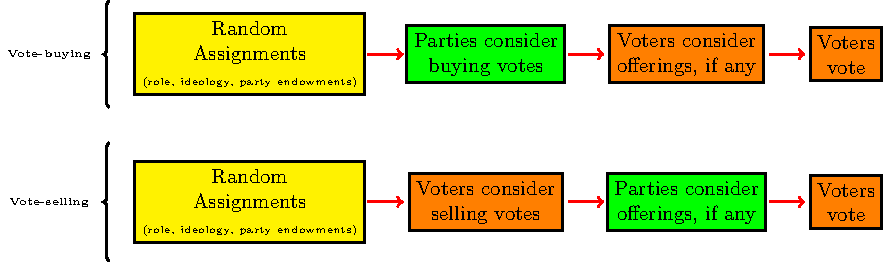
\includegraphics[scale=.7, center]{Experimental_Flow_Figure.pdf}
\caption{{\bf Experimental Flow.\label{experimental:design:fig}}\\\hspace{\textwidth} {\bf Note}: Note here.}\centering
\end{figure}




During the second stage of the first part, parties decide whether to go out and buy votes by making clientelist offerings. Experimental subjects playing the party role enter an amount of points, which ranges from zero to the maximum assigned budget. \todo{es asi? O ellos tienen que poner ``no quiero oferta''?} In the third stage voters evaluate whether to take that offer or not. They are also told that accepting the offer necessarily implies voting for that party (no defecting). In this regard, the third and fourth stage are in reality one stage.

The second part is the vote-selling portion of the experiment. This part is run during the same experimental session, but loading a separate \texttt{Ztree} program. Right after the first part is completed, experimental subjects are then asked to continue with the study. The part is exactly the same, except that this time voters are first-players: they get to offer parties an amount of points, and then, parties get to decide whether to take or reject that offer. 

The experimental currency 











\clearpage
\newpage
\pagenumbering{roman}
\setcounter{page}{1}
\printbibliography
\clearpage
\newpage



%%%%%%%%%%%%%%%%%%%%%%%%%%%%%%%%%%%%%%%%%%%%%%
% WORD COUNT
%%%%%%%%%%%%%%%%%%%%%%%%%%%%%%%%%%%%%%%%%%%%%%
\clearpage
\newpage
\pagenumbering{gobble}



\begin{center}
\vspace*{\stretch{1}}
\dotfill
\dotfill {\huge {\bf Word count}: 1,913} \dotfill
\dotfill
\vspace*{\stretch{1}}
\end{center}

\clearpage
\newpage

%%%%%%%%%%%%%%%%%%%%%%%%%%%%%%%%%%%%%%%%%%%%%%
% WORD COUNT
%%%%%%%%%%%%%%%%%%%%%%%%%%%%%%%%%%%%%%%%%%%%%%


% Online Appendix
%\newpage
%\section{Online Appendix}
%\pagenumbering{Roman}
%\setcounter{page}{1}



%% reset tables and figures counter
%\setcounter{table}{0}
%\renewcommand{\thetable}{OA\arabic{table}}
%\setcounter{figure}{0}
%\renewcommand{\thefigure}{OA\arabic{figure}}



%\section{Appendix}
%\pagenumbering{roman}
%\setcounter{page}{1}
%\newpage



\end{document}






